\newpage
\section{FUERZA}
\section{GALGAS EXTENSIOMETRICAS}
Las galgas extensométricas son sensores que miden la deformación de un objeto. Su funcionamiento se basa en el efecto piezorresistivo, donde la resistencia eléctrica del material cambia al ser sometido a esfuerzos mecánicos. Cuando se aplica una fuerza externa, el objeto se deforma, y esta deformación provoca una variación en la resistencia de la galga, que puede medirse y correlacionarse con la magnitud de la fuerza aplicada. Estos sensores son fundamentales en la medición de fuerzas, presiones y tensiones en diversas aplicaciones de ingeniería.\autoref{fig:GAL}
\begin{figure}[h]
	\centering
	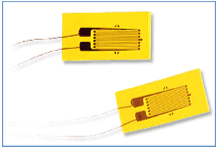
\includegraphics[width=0.3\linewidth]{img/GAL}
	\caption{Galgas }
	\label{fig:GAL}
\end{figure}

\section*{INTERRUPTOR DE EFECTO HALL}
Estos dispositivos detectan la presencia de un campo magnético. El efecto Hall se manifiesta cuando una corriente eléctrica que fluye a través de un semiconductor se ve afectada por un campo magnético perpendicular, generando una diferencia de potencial (voltaje Hall) transversal al flujo de corriente. Los interruptores de efecto Hall utilizan este principio para detectar campos magnéticos y, en consecuencia, activar o desactivar circuitos electrónicos. Son ampliamente utilizados en aplicaciones donde se requiere una detección precisa y sin contacto de posiciones o movimientos, como en sistemas de control de motores y dispositivos de seguridad.\autoref{fig:INTERRUPTOR HALL}
\begin{figure}[h]
	\centering
	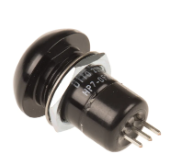
\includegraphics[width=0.3\linewidth]{img/INTERRUPTOR HALL}
	\caption{ Interruptor HALL }
	\label{fig:INTERRUPTOR HALL}
\end{figure}


